%%%%\%%%%%%%%%%%%%%%%%%%%%%%%%%%%%%%%%%%%%%%%%%%
%% Introduction aux Systèmes d'exploitation  %%
%%   * Historique                            %%
%%   * Principes fondamentaux                %%
%%   * Grandes classes de systèmes           %%
%%%%%%%%%%%%%%%%%%%%%%%%%%%%%%%%%%%%%%%%%%%%%%%

\title{Systèmes d'exploitation, 2ème année}
\subtitle{Fichiers et processus}

\author{Yves \textsc{Stadler}}\institute{Université Paul Verlaine - Metz}

\date{\today}

\begin{document}


%%
% Page de Titre
%%
\begin{frame}
\titlepage
\end{frame}

\def\sectitle{Les processus}
\section{\sectitle}

\begin{frame}{\sectitle}

\def\subsectitle{Définition}
\subsection{\subsectitle}


\begin{alertblock}{\subsectitle}
\begin{itemize}
    \item Entité associée par le noyau à l'exécution d'un programme. Un
    programme peut être exécuté pare un utilisateur et peut avoir plusieurs
    processus associés.
\end{itemize}
\end{alertblock}



\def\subsectitle{Hiérarchie des processus}
\subsection{\subsectitle}

\begin{columns}[b]

\column{.5\textwidth}
\begin{block}{\subsectitle}
\begin{itemize}
    \item Hiérarchie arborescente;
    \item Relation père-fils;
    \item Processus \textit{init} (pid: 1), racine;
    \item \textit{daemon} (cron, mémoire, messagerie, \dots);
    \item indépendants.
\end{itemize}
\end{block}

\column{.3\textwidth}
\begin{figure}
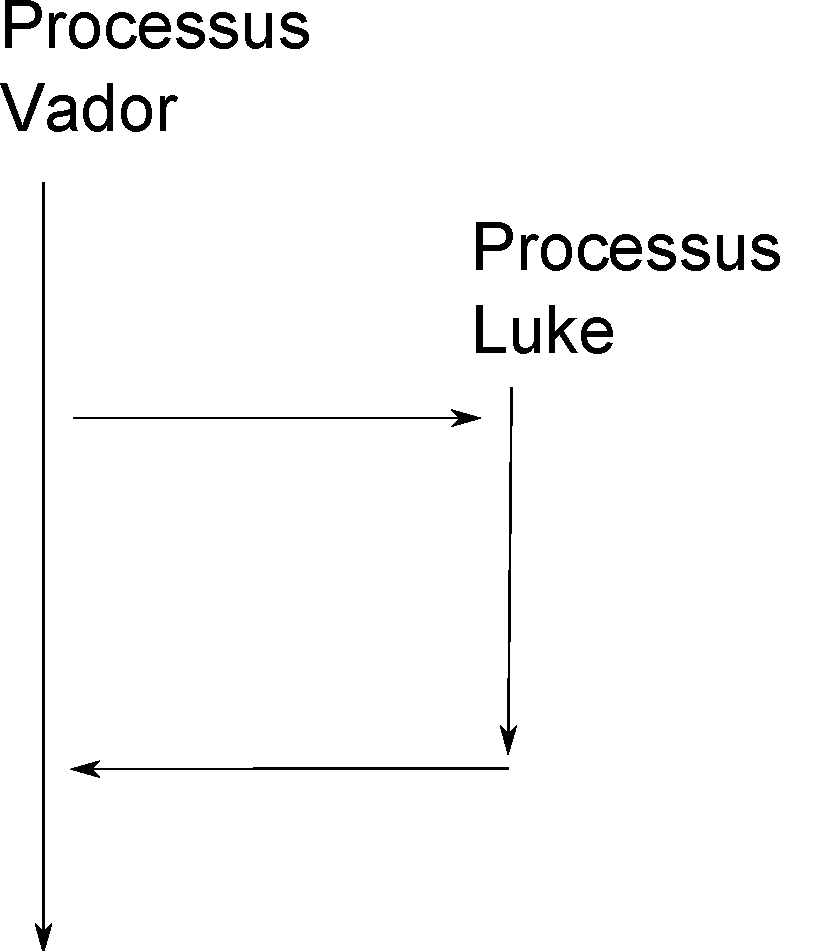
\includegraphics[width=\textwidth]{images/PereFils.pdf}
\end{figure}

\end{columns}

\end{frame}


\begin{frame}{\sectitle}
\def\subsectitle{Initialisation}
\subsection{\subsectitle}

\begin{block}{\subsectitle}
\begin{itemize}
    \item Le noyau est chargé par le \texttt{bootstrapping};
    \item Le noyau va résider en mémoire tant que la machine est allumée.
    \item Au démarrage le noyau exécute le processus \texttt{init} pid 1;
    \item \texttt{init} lit \texttt{/dev/tty} qui décrit les terminaux;
    \item \texttt{init} créer un fils pour chaque terminal et se met en veille;
    \item chaque fils exécute le programme \texttt{login}.
\end{itemize}
\end{block}
\end{frame}

\def\sectitle{Modes}
\section{\sectitle}

\begin{frame}{\sectitle}
\def\subsectitle{Deux espaces différents}
\subsection{\subsectitle}

\begin{block}{\subsectitle}
\begin{itemize}
    \item Espace usager: information du processus, fichiers ouverts, registre
    \item Espace kernel: fonction de tous les processus en appels système.
\end{itemize}
\end{block}

\end{frame}

%%%%%%%%%%%%%%%%%%%%%%%%%%%%%%%%%%%
\def\sectitle{Contexte}
\section{\sectitle}

\begin{frame}{\sectitle}

\def\subsectitle{Deux contextes différents}
\subsection{\subsectitle}

\begin{block}{\subsectitle}
\begin{itemize}
    \item Processus: le kernel opère pour le compte du processus (appels
    système);
    \item Système: le kernel gère les problèmes du système: interruptions
    périphérique, \dots
\end{itemize}
\end{block}
\end{frame}

\begin{frame}{\sectitle}
\begin{figure}
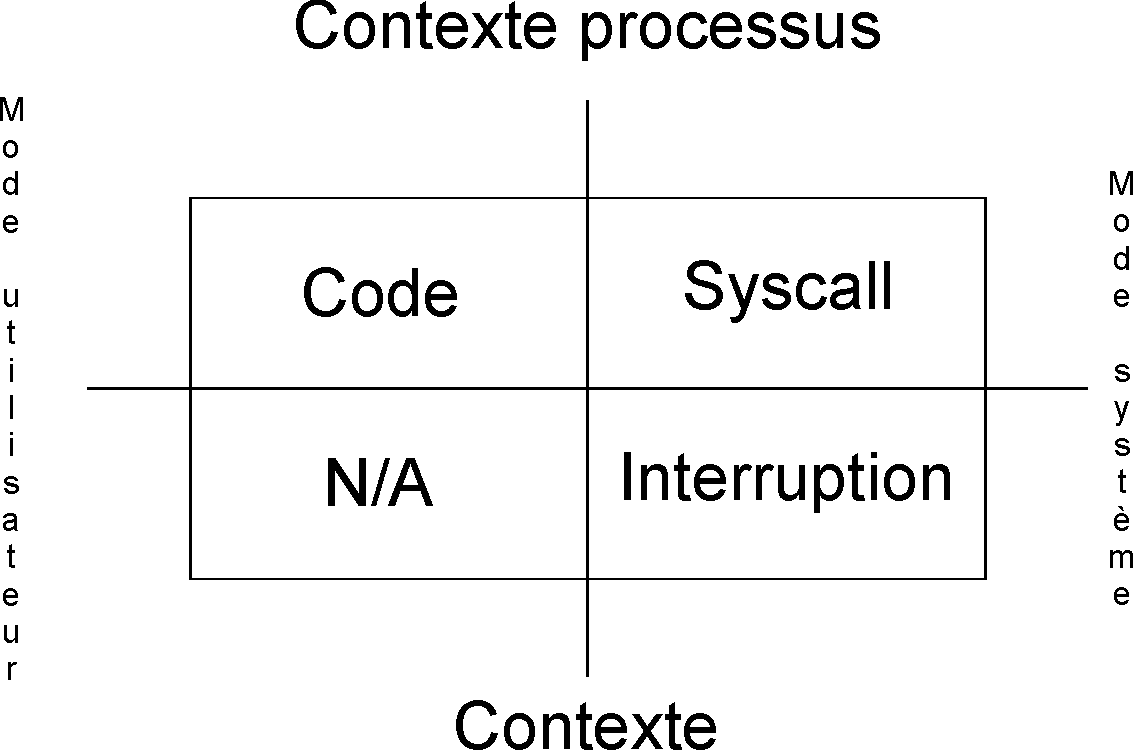
\includegraphics[width=.9\textwidth]{images/ContextMode.pdf}
\caption{Modes et contextes}
\end{figure}
\end{frame}

%%%%%%%%%%%%%%%%%%%%%%%%%%%%%%%%%%%
\def\sectitle{États d'un processus}
\section{\sectitle}

\begin{frame}{\sectitle}

\def\subsectitle{Définition}
\subsection{\subsectitle}

\begin{exampleblock}{\subsectitle}
\begin{itemize}
    \item Un processus peut se décrire comme une alternance de section actives,
    durant lesquelles des unités de temps CPU sont consommées, avec des attentes
    d'entrées sorties.
\end{itemize}
\end{exampleblock}

\def\subsectitle{Deux mécanismes de gestion}
\subsection{\subsectitle}

\begin{block}{\subsectitle}
\begin{itemize}
    \item Ordonnancement (\textit{scheduling}): choix des processus à activer;
    \item Synchronisation: gestion des ressources partagées;
    \item Le \textit{Process Control Block}: structure qui représente l'état
    d'un processus (lorsqu'il n'est pas en mémoire).
\end{itemize}
\end{block}

\end{frame}




%%%%%%%%%%%%%%%%%%%%%%%%%%%%%%%%%%%
\begin{frame}{\sectitle}
\begin{figure}
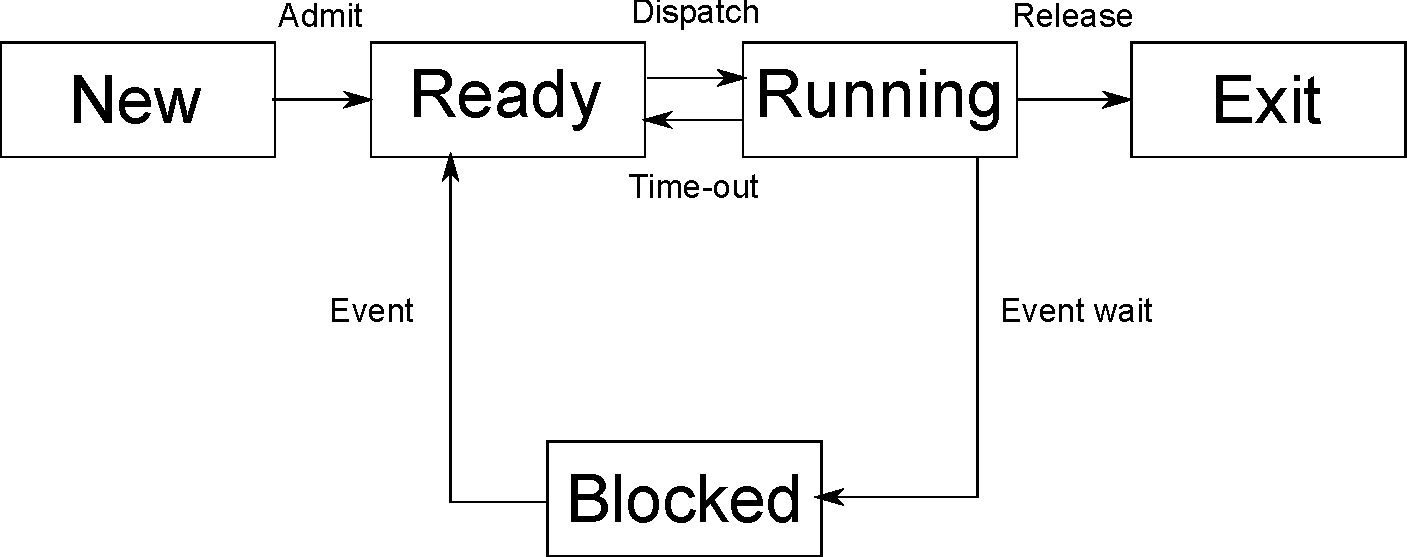
\includegraphics[width=.9\textwidth]{images/StateSimple.pdf}
\caption{État simplifié des processus}
\end{figure}
\end{frame}

%%%%%%%%%%%%%%%%%%%%%%%%%%%%%%%%%%%

\def\sectitle{Changement de contexte}
\section{\sectitle}

\begin{frame}{\sectitle}
\begin{figure}
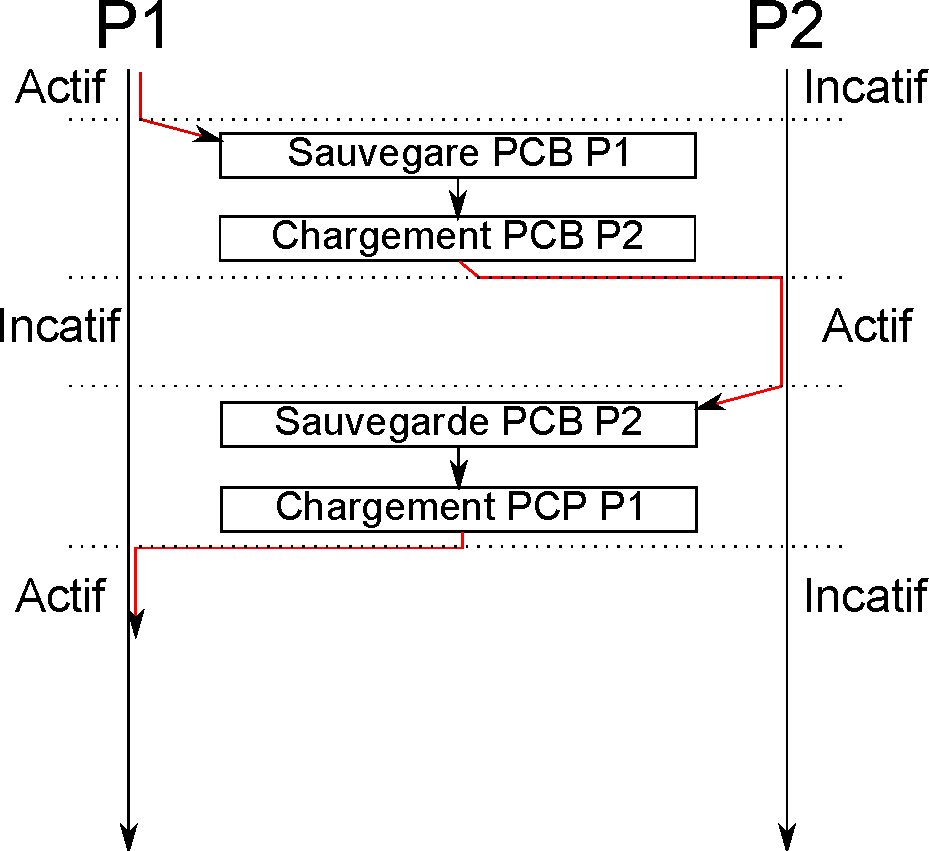
\includegraphics[width=.9\textwidth]{images/ContextChange.pdf}
\caption{Changement de contexte}
\end{figure}
\end{frame}

%%%%%%%%%%%%%%%%%%%%%%%%%%%%%%%%%%%
\def\sectitle{États d'un processus}
\section{\sectitle}
\begin{frame}{\sectitle}
\begin{figure}
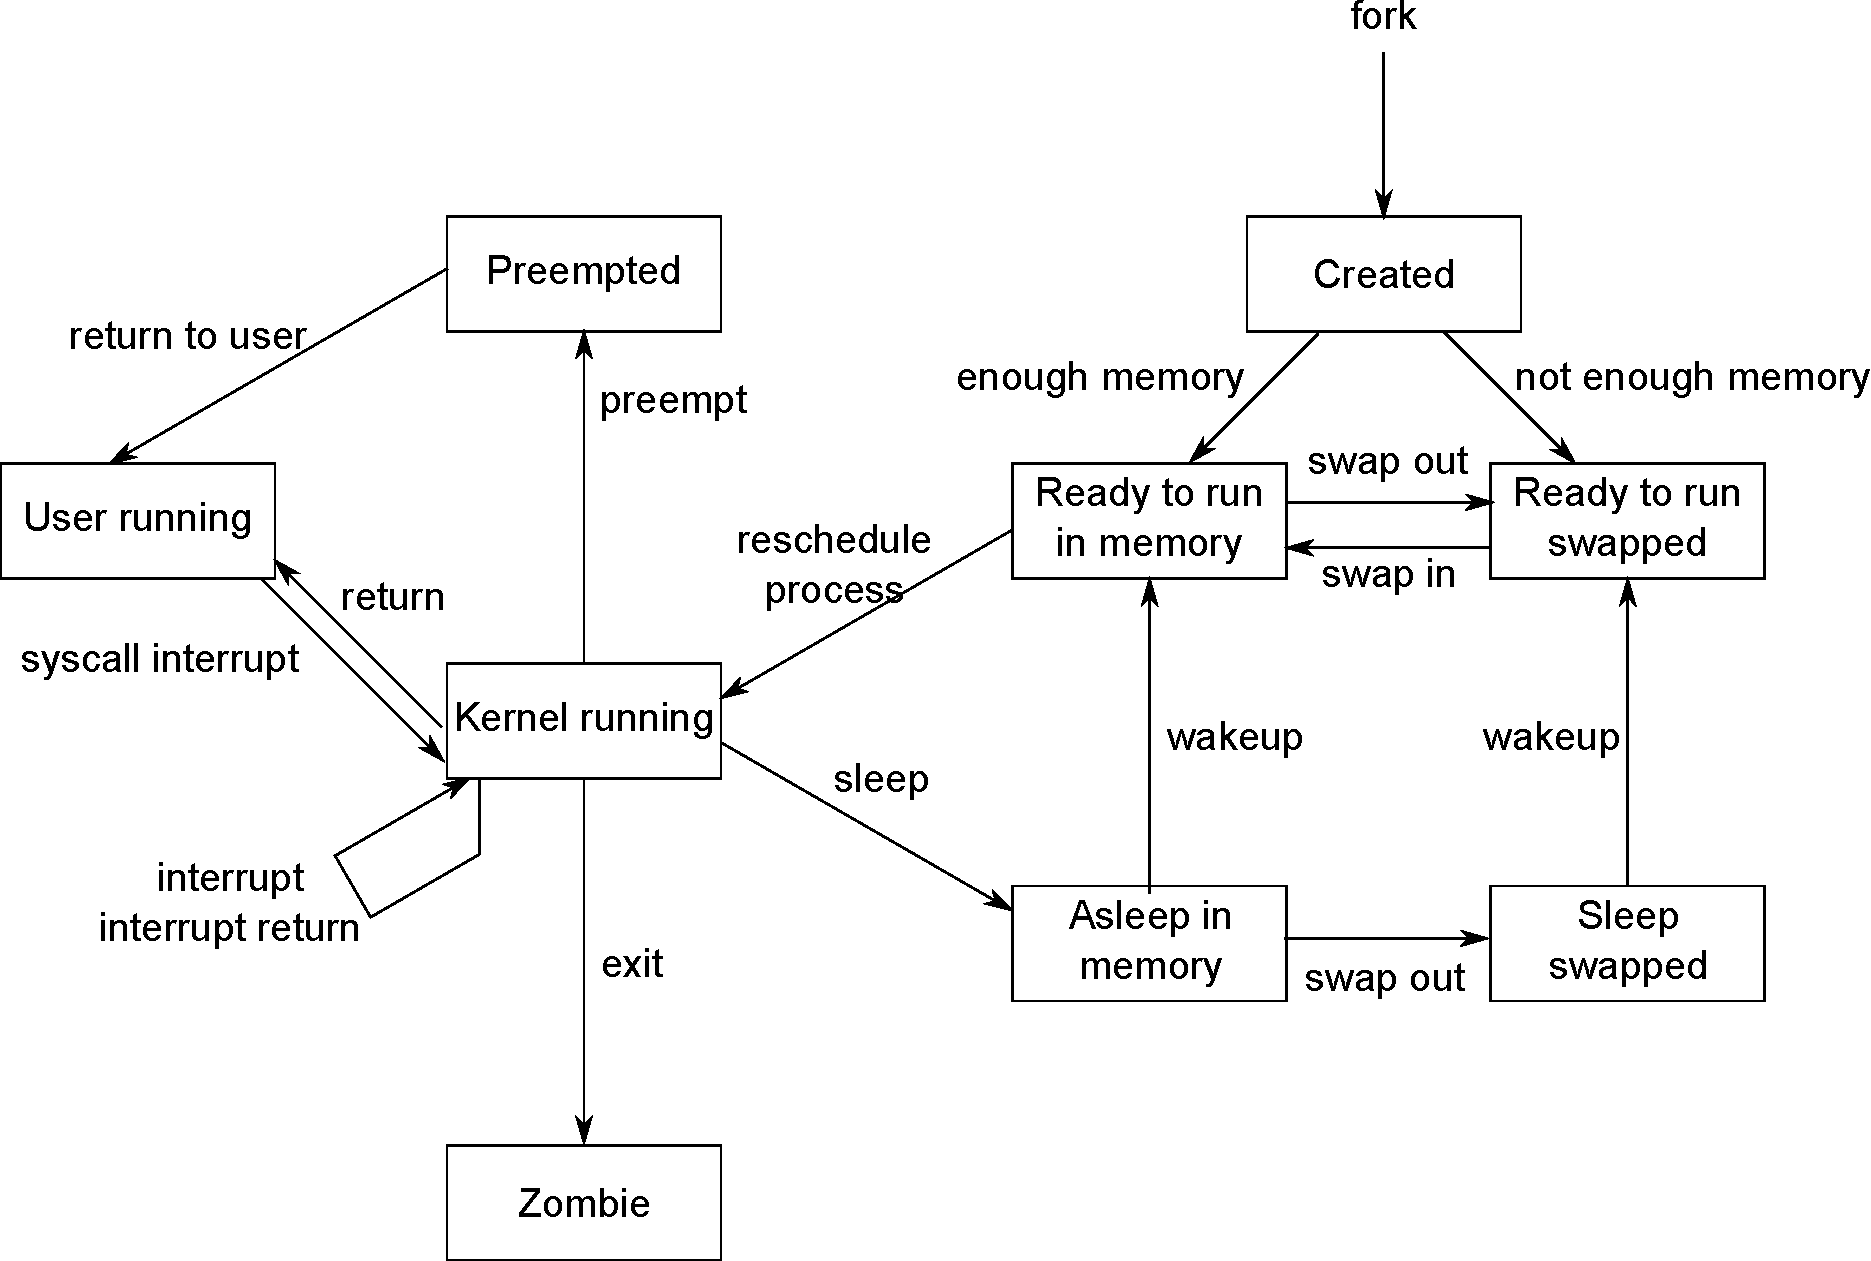
\includegraphics[width=.9\textwidth]{images/StateFull.pdf}
\caption{État d'un processus}
\end{figure}
\end{frame}



%%%%%%%%%%%%%%%%%%%%%%%%%%%%%%%%%%%
\def\sectitle{Primitives}
\section{\sectitle}

\begin{frame}{\sectitle}

\def\subsectitle{Création}
\subsection{\subsectitle}

\begin{block}{\subsectitle}
\begin{itemize}
    \item \texttt{fork()} (Retourne 0 dans le processus fils, pid de l'enfant
    dans le processus père);
    \item héritage de l'image mémoire;
    \item héritage de la table des fichiers ouverts;
    \item copie du PCB du père à l'emplacement du PCB du fils (seul différence
    les pid).
\end{itemize}
\end{block}

\def\subsectitle{Identité}
\subsection{\subsectitle}

\begin{block}{\subsectitle}
\begin{itemize}
    \item \texttt{getpid()} donne le numéro du processus en cours d'exécution;
    \item \texttt{getppid()} donne le numéro du père du processus en cours
    d'exécution.
\end{itemize}
\end{block}

\end{frame}
%%%%%%%%%%%%%%%%%%%%%%%%%%%%%%%%%%%

\def\sectitle{Les appels systèmes}
\section{\sectitle}

\begin{frame}{\sectitle}
\def\subsectitle{Processus}
\subsection{\subsectitle}

\begin{exampleblock}{\subsectitle}
\begin{itemize}
    \item \texttt{fork()} ;
    \item \texttt{kill()} ;
    \item \texttt{waitpid()} ;
    \item \texttt{alarm()} ;
    \item \texttt{pause()} ;
\end{itemize}
\end{exampleblock}

\def\subsectitle{Répertoires}
\subsection{\subsectitle}

\begin{exampleblock}{\subsectitle}
\begin{itemize}
    \item \texttt{mkdir()} créer un répertoire;
    \item \texttt{chdir()} change de répertoire;
\end{itemize}
\end{exampleblock}

\end{frame}

\begin{frame}{\sectitle}
\def\subsectitle{Fichier}
\subsection{\subsectitle}

\begin{exampleblock}{\subsectitle}
\begin{itemize}
    \item \texttt{creat()} créer un fichier;
    \item \texttt{open()} ouvre un descripteur de fichier en lecture ;
    \item \texttt{close()} ferme le descripteur de fichier ;
    \item \texttt{read()} read the file descriptor ;
    \item \texttt{write()} write in the file descriptor ;
\end{itemize}
\end{exampleblock}

\def\subsectitle{Mémoire}
\subsection{\subsectitle}

\begin{exampleblock}{\subsectitle}
\begin{itemize}
    \item \texttt{malloc()} allocation de mémoire;
    \item \texttt{free()} libération de la mémoire;
\end{itemize}
\end{exampleblock}

\end{frame}
%%%%%%%%%%%%%%%%%%%%%%%%%%%%%%%%%

\def\sectitle{Ordonnancement}
\section{\sectitle}

\begin{frame}{\sectitle}
\def\subsectitle{Rôle de l'ordonnanceur}
\subsection{\subsectitle}

\begin{block}{\subsectitle}
\begin{itemize}
    \item Choisir les processus qui vont accéder au CPU
    \item Lorsqu'il faut gérer de la mémoire virtuelle, l'ordonnancement se
    fait à deux niveaux
    \begin{itemize}
        \item Haut niveau: sélection les prochain processus à charger en mémoire
        \item Bas niveau : sélectionne le processus qui accède au CPU parmi ceux
        qui sont prêts.
    \end{itemize}
\end{itemize}
\end{block}

\def\subsectitle{Les files d'attentes}
\subsection{\subsectitle}

\begin{block}{\subsectitle}
\begin{itemize}
    \item Un ordonnanceur gère plusieurs files d'attentes: 
    \begin{itemize}
        \item Processus prêts;
        \item Processus en attente d'entrée / sortie.
    \end{itemize}
    \item La question est: comment insère-t-on un processus dans une file et
    \item comment un processus passe d'une file au CPU.
\end{itemize}
\end{block}
\end{frame}

\def\sectitle{Traitement par flots}
\section{\sectitle}

\begin{frame}{\sectitle}
\def\subsectitle{Batch processing}
\subsection{\subsectitle}

\begin{columns}[c]

\column{.4\textwidth}
\begin{block}{\subsectitle}
\begin{itemize}
    \item Pas de répartiteur de bas niveau (ou répartiteur trivial)
    \item Lorsqu'une opération d'entrée sortie est déclenchées, le CPU est
    inactif.
\end{itemize}
\end{block}

\column{.6\textwidth}
\begin{figure}
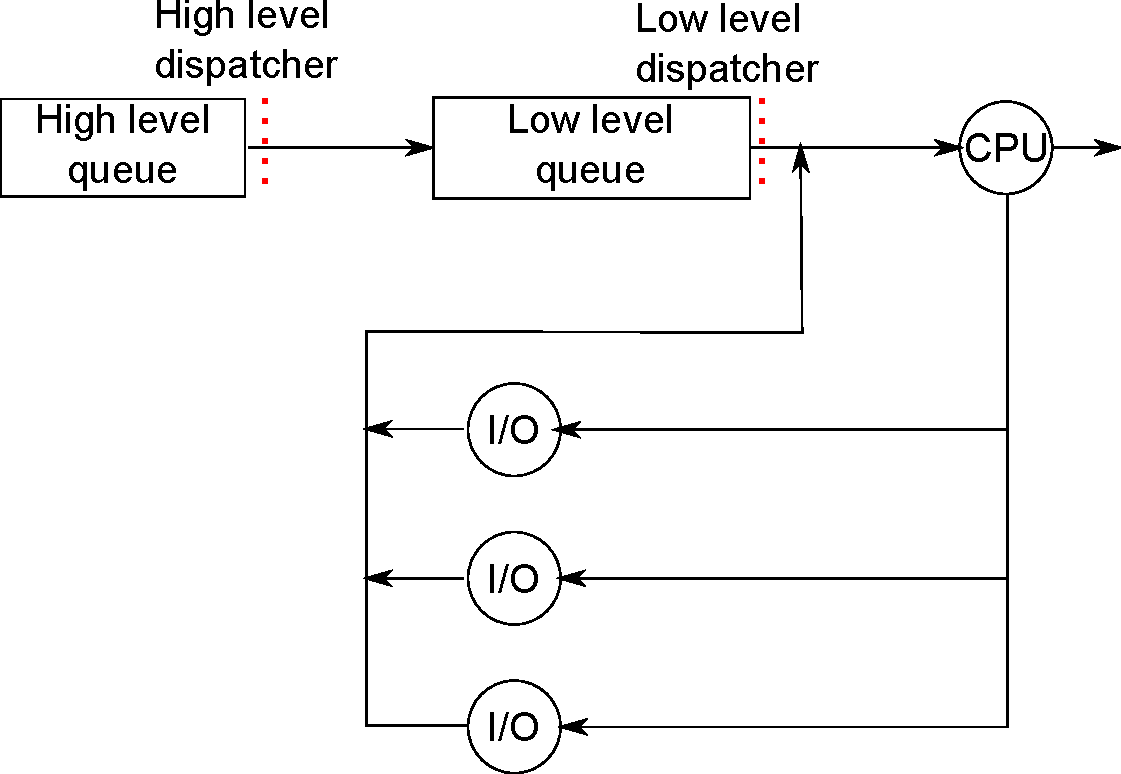
\includegraphics[width=\textwidth]{images/batchDispatching.pdf}
\caption{État d'un processus}
\end{figure}

\end{columns}

\end{frame}

\def\sectitle{Multi-programmation}
\section{\sectitle}

\begin{frame}{\sectitle}
\def\subsectitle{Multi-programmation}
\subsection{\subsectitle}

\begin{columns}[c]
\column{.4\textwidth}
\begin{block}{\subsectitle}
\begin{itemize}
    \item Lorsqu'une opération d'entrée sortie est déclenchées, le CPU est
    libéré;
    \item les processus qui termine une entrée sortie sont remis dans la file.
\end{itemize}
\end{block}

\column{.6\textwidth}
\begin{figure}
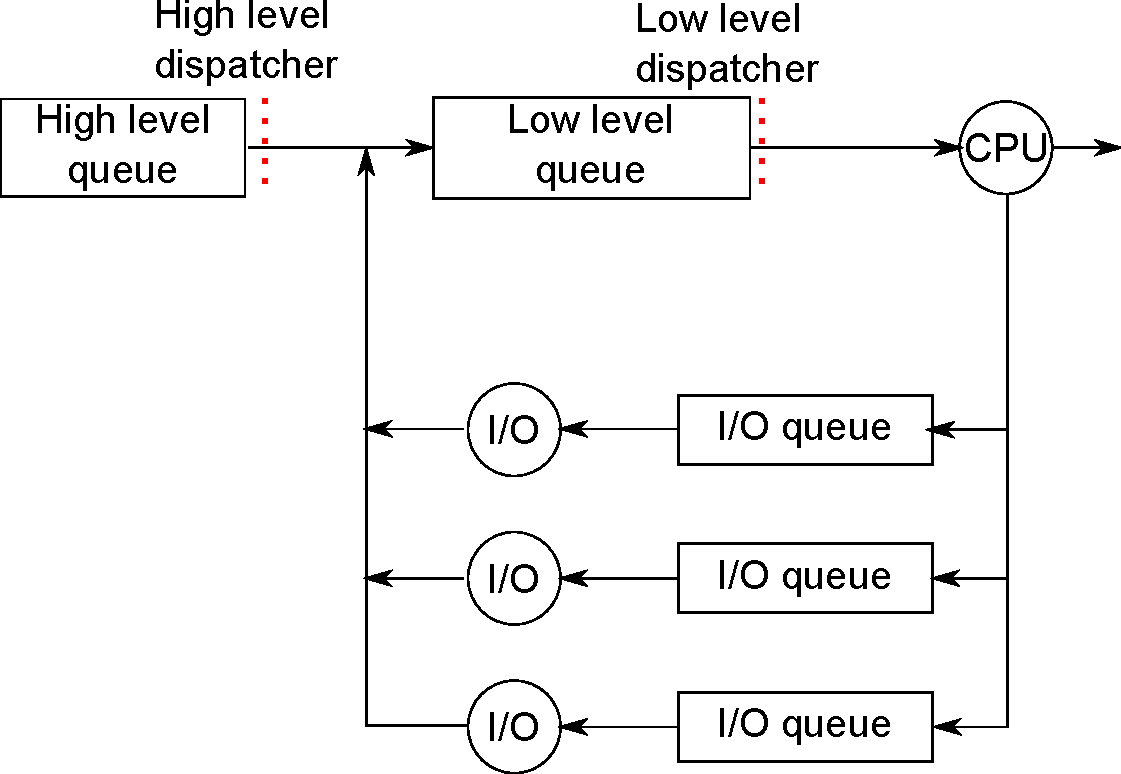
\includegraphics[width=\textwidth]{images/multiprogDispatching.pdf}
\caption{État d'un processus}
\end{figure}
\end{columns}

\end{frame}

\def\sectitle{Temps partagé}
\section{\sectitle}
\begin{frame}{\sectitle}
\def\subsectitle{Time sharing}
\subsection{\subsectitle}

\begin{columns}[c]
\column{.4\textwidth}
\begin{block}{\subsectitle}
\begin{itemize}
    \item Chaque processus dispose d'un certain temps de CPU;
    \item les processus qui dépasse ce délai sont remis dans la file;
    \item On appelle quantum de temps la durée maximale allouée à chaque
    processus.
\end{itemize}
\end{block}

\column{.6\textwidth}
\begin{figure}
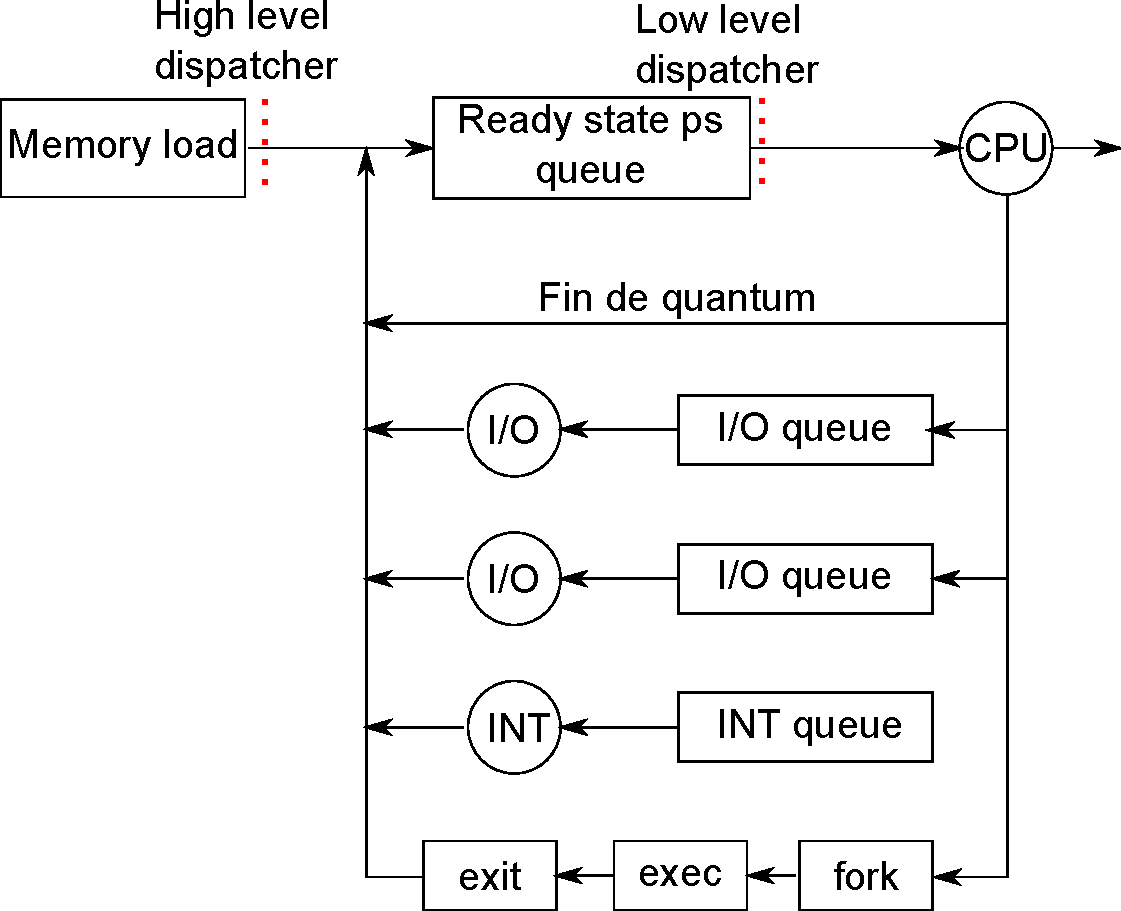
\includegraphics[width=\textwidth]{images/timesharingDispatching.pdf}
\caption{État d'un processus}
\end{figure}
\end{columns}

\end{frame}


\def\sectitle{Mémoire virtuelle}
\section{\sectitle}
\begin{frame}{\sectitle}
\def\subsectitle{Virtual memory}
\subsection{\subsectitle}

%\begin{block}{\subsectitle}
%\begin{itemize}
%    \item Chaque processus dispose d'un certain temps de CPU;
%    \item les processus qui dépasse ce délai sont remis dans la file;
%    \item On appelle quantum de temps la durée maximale allouée à chaque
%    processus.
%\end{itemize}
%\end{block}

\begin{figure}
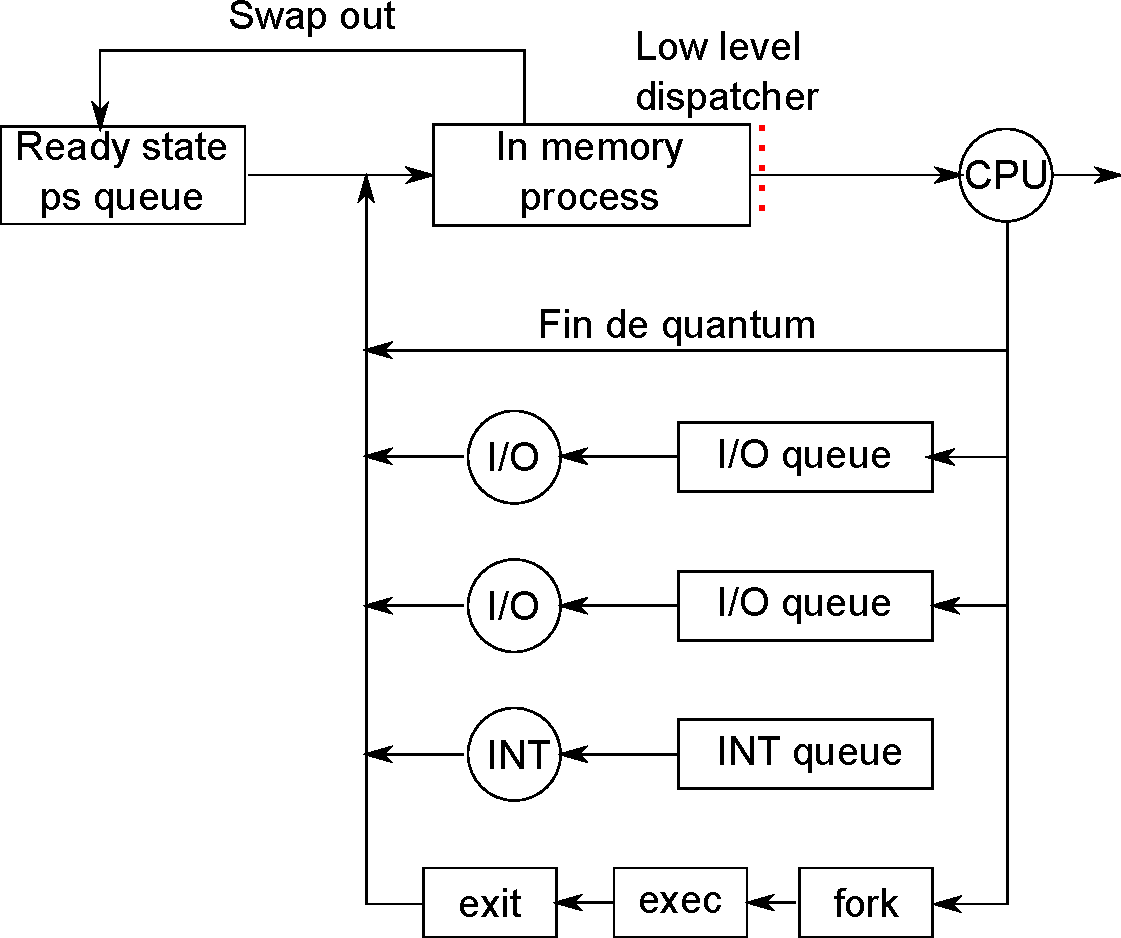
\includegraphics[width=.7\textwidth]{images/virtualmemoryDispatching.pdf}
\caption{État d'un processus}
\end{figure}

\end{frame}




%%%%%%%%%%%%%%%

\def\sectitle{Les algorithmes d'ordonnancement}
\section{\sectitle}

\begin{frame}{\sectitle}
\def\subsectitle{Plan}
\subsection{\subsectitle}

\begin{block}{\subsectitle}
\begin{itemize}
    \item Critères d'ordonnancement;
    \item First In First Out;
    \item Shortest Job First;
    \item Round Robin;
    \item Listes multiples;
    \item Évaluations.
\end{itemize}
\end{block}

\end{frame}


\def\sectitle{Les critères}
\section{\sectitle}

\begin{frame}{\sectitle}

\def\subsectitle{Minimiser, maximiser ?}
\subsection{\subsectitle}
\begin{block}{\subsectitle}
\begin{itemize}
    \item On peut minimiser
    \begin{itemize}
        \item le temps entre soumission et fin d'une tâche
        \item le temps de passage en file bas niveau;
        \item le temps d'exécution des entrées sorties.
    \end{itemize}
    \item maximiser:
    \begin{itemize}
        \item Le taux d'activité du CPU;
        \item Le nombre de processus traités par unités de temps.
    \end{itemize}
\end{itemize}
\end{block}
\end{frame}

\begin{frame}{\sectitle}

\def\subsectitle{Classes d'ordonnanceurs}
\subsection{\subsectitle}

\begin{block}{\subsectitle}
\begin{itemize}
    \item Non-préemptifs: un processus libère le CPU quand il n'en a plus
    besoin;
    \item Préemptifs: l'utilisation du CPU est limitée dans le temps.
\end{itemize}
\end{block}

\begin{exampleblock}{\subsectitle}
\begin{itemize}
    \item Préemptif: Unix, WinNT, BeOS, Win2000, MacOS X (et suivants);
        \item Non préemptif: MacOS, Win9X, Millenium.
\end{itemize}
\end{exampleblock}

\end{frame}

\def\sectitle{First In First Out}
\section{\sectitle}

\begin{frame}{\sectitle}

\def\subsectitle{FIFO}
\subsection{\subsectitle}

\begin{block}{\subsectitle}
\begin{itemize}
    \item Principe d'une file standard, les éléments rentre à la suite de tous
    les processus déjà présents;
    \item Le processus qui n'a plus de prédécesseur est la tête de la file et
    est élu à la prochaine sélection.
\end{itemize}
\end{block}


\begin{figure}

\includegraphics[width=\textwidth]{images/FIFO.pdf}
\end{figure}

\end{frame}


\def\sectitle{Shortest Job First}
\section{\sectitle}

\begin{frame}{\sectitle}
\def\subsectitle{SJF}
\subsection{\subsectitle}

\begin{block}{\subsectitle}
\begin{itemize}
    \item La tâche la plus courte à la priorité
    \item Les processus sont triés en fonction du nombre d'unités CPU qu'il
    requiert.
    \item En cas d'égalité : FIFO.
    \item Comment connait-on le temps CPU des processus?
\end{itemize}
\end{block}


\def\subsectitle{Estimation du temps CPU}
\subsection{\subsectitle}

\begin{block}{\subsectitle}
\begin{itemize}
    \item Demander à l'utilisateur;
    \item Estimer à partir de l'historique : $p_{n+1} = a*t_{n}+(1-a)*p_{n}$
    \item SJF avec priorité
\end{itemize}
\end{block}
\end{frame}

\begin{frame}{\sectitle}
\def\subsectitle{Problème}
\subsection{\subsectitle}

\begin{alertblock}{\subsectitle}
\begin{itemize}
    \item Comment éviter les famines?
\end{itemize}
\end{alertblock}


\begin{exampleblock}{\subsectitle}
\begin{itemize}
    \item Ajouter un vieillissement automatique des processus.
\end{itemize}
\end{exampleblock}
\end{frame}


\def\sectitle{Round Robbin}
\section{\sectitle}

\begin{frame}{\sectitle}
\def\subsectitle{Principe}
\subsection{\subsectitle}

\begin{exampleblock}{\subsectitle}
\begin{itemize}
    \item FIFO préemptif
    \item Utilisation d'un quantum de temps
    \item Libération du CPU lors des entrées sorties, de la fin du processus ou
    lorsque le quantum est épuisé.
\end{itemize}
\end{exampleblock}

\def\subsectitle{Quel quantum choisir}
\subsection{\subsectitle}

\begin{alertblock}{\subsectitle}
\begin{itemize}
    \item Trop court: important changement de contexte qui pénalise l'efficacité
    du système;
    \item Trop long: les processus court sont pénalisés;
    \item Infini : on a une FIFO;
    \item Unix utilise 100ms.
\end{itemize}
\end{alertblock}

\end{frame}

\end{document}
